\documentclass[a4paper]{article}
\usepackage[utf8x]{inputenc}
\usepackage[T1,T2A]{fontenc}
\usepackage[russian]{babel}
\usepackage{hyperref}
\usepackage{indentfirst}
\usepackage{listings}
\usepackage{color}
\usepackage{here}
\usepackage{array}
\usepackage{multirow}
\usepackage{graphicx}

\usepackage{caption}
\renewcommand{\lstlistingname}{Программа} % заголовок листингов кода

\usepackage{listings}
\lstset{ %
extendedchars=\true,
keepspaces=true,
language=C,						% choose the language of the code
basicstyle=\footnotesize,		% the size of the fonts that are used for the code
numbers=left,					% where to put the line-numbers
numberstyle=\footnotesize,		% the size of the fonts that are used for the line-numbers
stepnumber=1,					% the step between two line-numbers. If it is 1 each line will be numbered
numbersep=5pt,					% how far the line-numbers are from the code
backgroundcolor=\color{white},	% choose the background color. You must add \usepackage{color}
showspaces=false				% show spaces adding particular underscores
showstringspaces=false,			% underline spaces within strings
showtabs=false,					% show tabs within strings adding particular underscores
frame=single,           		% adds a frame around the code
tabsize=2,						% sets default tabsize to 2 spaces
captionpos=b,					% sets the caption-position to bottom
breaklines=true,				% sets automatic line breaking
breakatwhitespace=false,		% sets if automatic breaks should only happen at whitespace
escapeinside={\%*}{*)},			% if you want to add a comment within your code
postbreak=\raisebox{0ex}[0ex][0ex]{\ensuremath{\color{red}\hookrightarrow\space}},
texcl=true,
}

\usepackage[left=2cm,right=2cm,
top=2cm,bottom=2cm,bindingoffset=0cm]{geometry}


\begin{document} % начало документа
\raggedbottom
%\begin{titlepage}	% начало титульной страницы

	\begin{center}		% выравнивание по центру

		\large Санкт-Петербургский Политехнический Университет Петра Великого\\
		\large Институт компьютерных наук и технологий \\
		\large Кафедра компьютерных систем и программных технологий\\[6cm]
		% название института, затем отступ 6см
		
		\huge Название предмета\\[0.5cm] % название работы, затем отступ 0,5см
		\large Отчет по лабораторной работе №1\\[0.1cm]
		\large Тема работы\\[5cm]

	\end{center}


	\begin{flushright} % выравнивание по правому краю
		\begin{minipage}{0.25\textwidth} % врезка в половину ширины текста
			\begin{flushleft} % выровнять её содержимое по левому краю

				\large\textbf{Работу выполнил:}\\
				\large Петров В.Д.\\
				\large {Группа:} 43501/4\\
				
				\large \textbf{Преподаватель:}\\
				\large Ицыксон В.М.

			\end{flushleft}
		\end{minipage}
	\end{flushright}
	
	\vfill % заполнить всё доступное ниже пространство

	\begin{center}
	\large Санкт-Петербург\\
	\large \the\year % вывести дату
	\end{center} % закончить выравнивание по центру

\thispagestyle{empty} % не нумеровать страницу
\end{titlepage} % конец титульной страницы

\vfill % заполнить всё доступное ниже пространство



% Содержание
%\tableofcontents
%\newpage
\title{Сравнение качества построения карты глубины при использовании различных калибровочных моделей сверхширокоугольных объективов}
\author{Пантелеев М.}
\institute{Санкт-Петербургский Политехнический Университет Петра Великого
\email{panteleev.md@edu.spbstu.ru}}
\maketitle

\begin{abstract}
	
	Пишу здесь на всякий случай, потому что прошлый раз мой комментарий на сайте Вы, кажется, не увидели. 
	Мы с Виктором Витальевичем исследовали модели камер в этом семестре и решили опубликовать про это статью, которую
	я и сюда мог сдать (ну и статья с первого семестра, в общем-то, в тупике). Но у меня возникли проблемы с некоторыми моделями, у него со свободным временем, ещё и дедлайны 
	как-то раньше ожидаемого случились, в итоге эксперименты проведены, но написать пока не успели. Этот документ - мой ранний
	 черновик этой статьи. Здесь есть проблемы, картинки надо будет менять, эксперимент в конце переделывать, но 
	на данный момент это выглядит так.

	Камеры "рыбий глаз" имеют большой потенциал длч применения в робототехнике. Одним из таких применений может быть поиск глубины и построение карт для задач автономной
	навигации. Однако чтобы реализовать этот потенциал, должна быть использована точная модель камеры. В этой статье исследуются актуальные калибровочные модели 
	сверхширокоугольных камер и их применимости в системах стереозрения. Приведены оценки точности построения карты глубины для каждой модели. Проведённые эксперименты 
	позволили определить самую оптимальную по нескольким параметрам модель. 

\end{abstract}

\section{Введение}

За последние годы был достигнут существенный прогресс в доступности и точности сенсоров, позволяющих мобильным роботам 
проводить оценку окружающего пространства. Такие информационно-измерительные устройства как лидары, сонары и стереокамеры
 стали основным источником информации для алгоритмов автономной навигации и локализации. Тем не менее в роботах по-прежнему 
присутствуют телевизионные системы, так как они дают наиболее легко воспринимаемую информацию для оператора в случаях, когда 
его вмешательство необходимо. "Обычные" камеры, описываемые перспективной проекцией, дают изображение, понятное для 
восприятия и обработки, но покрывают зачастую слишком маленькую область пространства. Однако такие изображения в меньшей степени 
пригодны для применения в алгоритмах автономной навигации и локализации в виду того, что видят те или иные особенности окружающего
пространства в среднем более короткие промежутки времени \cite{stereo_slam}. 

Для достижения большего поля зрения могут быть использованы катадиоптрические системы, состоящие из выгнутого зеркала и 
перспективной камеры. Однако такой метод не всегда применим, так как система получается громоздкой и имеет "мёртвую зону" посередине 
кадра, как видно на рисунке \ref{pic:wideangle} (а). Наконец, можно использовать камеры "рыбий глаз" (англ. fisheye-camera), 
позволяющие с помощью специальной системы линз одним кадром покрыть угловое поле свыше $180^\circ$. В сравнении с 
катадиоптрическими они обладают большей полезной областью кадра, как видно на рисунке \ref{pic:wideangle} (б). %% можно ли так говорить? 
% stereo_slam: https://www.researchgate.net/publication/221786166_Stereo_Vision_Based_SLAM_Issues_and_Solutions

\begin{figure}[H]
	\begin{center}
		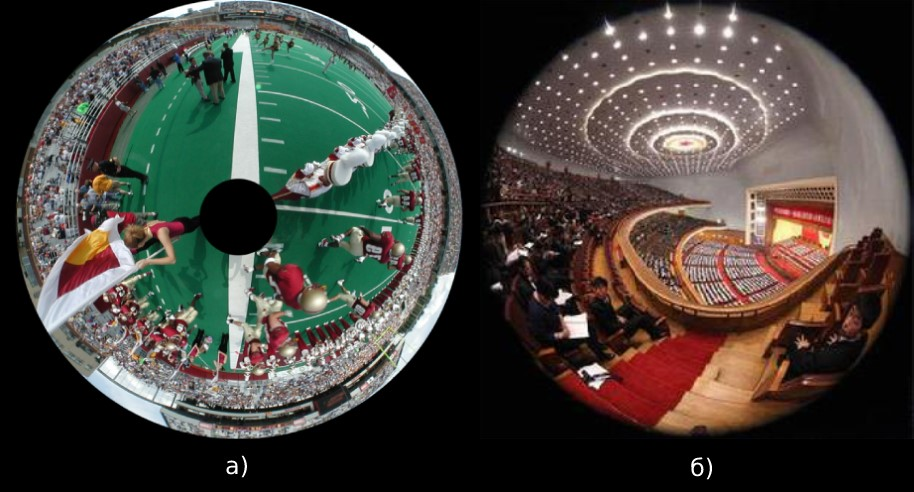
\includegraphics[scale=0.5]{pics/wideangle.jpg}
		\caption{Сравнение изображений с разных типов камер} 
		\label{pic:wideangle} % название для ссылок внутри кода
	\end{center}
\end{figure}

При этом, как видно по изображению, сверхшироукольные объективы накладывают на изображение заметные искажения.
Обычно принято выделять два вида искажений: тангенциальные и радиальные, но в данном случае тангенциальные принебрежимы по сравнению
 с радиальными и далее рассматриваться не будут. Устранение этих искажений является важной задачей, так как её решение позволяет 
 нивилировать недостатки сверхширокоугольных объективов и применять их для чувствительных к точности передачи формы объектов в кадре задач.

 Одной из таких задач является стереозрение. Несмотря на существование методов, позволяющих оценивать глубину по полным fisheye-снимкам \cite{singlecamrev}, 
классические методы, требующие ректификации, всё ещё остаются самыми доступными и производительными \cite{disparity_review}. Построив систему стереозрения на 
основе ортогонально расположенных сверхширокоугольных камер, можно получить ряд преимуществ перед традиционными камерами. Для этого 
сначала нужно выбрать модель искажений, наиболее точно описывающую данные линзы. \pdfcomment{[здесь бы сослаться на самого себя, но пока не на что,
и тогда, получается, что принцип этой системы тоже надо бы описать].}

Разработку и первоначальные испытания алгоритма стереозрения целесообразно проводить в виртуальной среде. Оптическая система была смоделирована 
в виртуальной среде с применением игрового движка Unity и плагина ZybrVR Dome Tools \cite{dome_tools}. Благодаря этому появляется возможность моделировать  %% TODO: что-то ещё про виртуальный опыт 
оптические системы разной конфигурации и иметь точную информацию о геометриии в кадре. 

\subsection{Модели камер "рыбий глаз"}

Сверхширокоугольные линзы изготавливают, закладывая разные виды проекций \cite{projections}, но 
но реальные линзы не всегда в точности соответствуют им, поэтому для более точного описания принято использовать модели дисторсии
 на основе других функций.
Определим основные обозначения. Модель проекции для камеры это функция (обычно обозначаемая $\pi_c(\cdot )$), которая моделирует преобразование 
из точки трёхмерного пространства ($P=[x_c, y_c, z_c]^T$) в поле зрения камеры в точку на плоскости изображения ($p=[u, \nu]^T$).Единичная            % не совсем единичная 
полусфера $S$ с центром в точке $O_c$ описывает поле зрения. На ней также лежит точка $P_C$, являющаяся результатом обратной проекции $\pi^{-1}_c({p})$.
Угол $\theta$ является углом падения для рассматриваемой точки, а угол $\phi$ откладывается между положительным направлением оси $u$ и $O_{i}{p}$. 
% TODO: переписать текст выше более правильным способом
\addimghere{pics/projection_geometry}{0.5}{Схема проекции точки трёхмерного пространства в точку на изображении}{pic:fy_geom}

Основными критериями выбора моделей были: пригодность для моделирования 
сверхширокоугольных линз, простота калибровки и распространённость. Существует несколько программных пакетов, позволяющих автоматически калибровать камеры. 
Это kalibr (модели Канналы-Брандта, Скарамуззы, Двух Сфер), OdoCamCalib (модели Мея и Канналы-Брандта), OpenCV (модели Канналы-Брандта и Брауна) и MATLAB 
(модели Скарамуззы и Брауны). Таким образом, далее будут рассмотрены основные модели камер, отобранные для сравнения. 

\subsubsection{Модель Канналы-Брандта}

Модель Канналы и 
Брандта \cite{opencv_model} реализована в частности OpenCV и описывает радиальные искажения через угол падения луча света на линзу, а не расстояние  
от центра изображения до места падения, как это делалось в более ранних моделях. Авторы посчитали, что для описания типичных искажений достаточно 
пяти членов полинома. Таким образом, указанную модель можно записать следующими уравнениями:

\begin{equation}
\begin{aligned}
	\pi(\mathbf{x}, \mathbf{i}) &=\left[\begin{array}{l}
	f_{x} d(\theta) \\
	f_{y} d(\theta)
	\end{array} \frac{x}{r}\right]+\left[\begin{array}{c}
	c_{x} \\
	c_{y}
	\end{array}\right] \\
	r &=\sqrt{x^{2}+y^{2}} \\
	\theta &=\operatorname{atan} 2(r, z) \\
	d(\theta) &=\theta+k_{1} \theta^{3}+k_{2} \theta^{5}+k_{3} \theta^{7}+k_{4} \theta^{9}
\end{aligned}
\end{equation}

Калибровка камеры по этой модели произведена с помощью библиотеки OdoCamCalib, средня ошибка перепроецирования 
составила 0.102 пикселя. \pdfcomment{mean reprojection error}

\subsubsection{Модель Скарамуззы}

Также большое распространение получила модель Скарамуззы \cite{scaramuzza}, которая легла в основу Matlab Omnidirectional 
Camera Calibration Toolbox, что позволяет быстро и удобно производить калибровку параметров модели.  Она связывает точки 
на изображении с соответствующей им точкой в координатах камеры следующим образом:

\begin{equation}	
    \pi^{-1}(\mathbf{u}, \mathbf{i}) = \lambda \begin{pmatrix}u\\v\\a_0 + a_2 r^2 + a_3 r^3 + a_4 r^4\end{pmatrix},
    %\delta r = k_1\theta + k_2\theta^3 + k_3\theta^5 + k_4\theta^7 + ... + k_n\theta^{n+1}
    \label{eqn:scaramuzza}
\end{equation}
где  $r$ - расстояние от спроектированной точки до центра изображения; $f$ - фокусное расстояние; $\lambda$ - масштабный коэффициент.

Однако для устранения искажений необходима прямая проекция, которая не выражается в явном виде  и находится методом 
Ньютона, что негативно сказывается не результате проекции. \pdfcomment{ проверить точность формулировок }

Средня ошибка перепроецирования составила 0.121 пикселей. %% + ошибка схождения 

\subsubsection{Модель Мея}

Модель Мея \cite{mei} изначально была создана для более эффективного моделирования катадиоптрических камер, но оказалась также весьма
пригодной и для fisheye-камер. 

\begin{equation}
\pi(\mathbf{x}, \mathbf{i})=\left[\begin{array}{l}
	f_{x} \frac{x}{\alpha d+(1-\alpha) z} \\
	f_{y} \frac{y}{\alpha d+(1-\alpha) z}
	\end{array}\right]+\left[\begin{array}{l}
	c_{x} \\
	c_{y}
	\end{array}\right]
\end{equation}

Калибровка камеры по этой модели произведена с помощью библиотеки OdoCamCalib, средня ошибка перепроецирования 
составила 0.099 пикселя.

\subsubsection{Atan}

Эта модель представляет из себя идеальную эквидистантную fisheye-проекцию, которая заложена в использованную виртуальную широкоугольную камеру. 
Она добавлена к сравнению как эталонный способ устранения искажений из предположения, что с ней результаты стереосопоставления будут 
самыми лучшими.  

\begin{equation}
	\pi(\mathbf{x}, \mathbf{i})=\left[\begin{array}{l}
		f_{x} \frac{\theta}{ \sqrt{ \frac{y^2}{x^2} + 1 }} \\
		f_{y} \frac{\theta}{ \sqrt{ \frac{x^2}{y^2} + 1 }}
		\end{array}\right]+\left[\begin{array}{l}
		c_{x} \\
		c_{y}
		\end{array}\right]
	\end{equation}

Кроме этой проекции для сравнения в экспериментах присутствуют дву идеальные камеры без искажений, направленные
ровно в том же направлении, в котором будет производиться устранение  искажений.  
%Таким образом, параметры всех моделей, используемых в сравнении, представлены в таблице \ref{tab:params}.

\pdfcomment{добавить таблицу}

\subsection{Построение стереопары}

Наиболее сильные искажения на изображении "рыбий глаз" возникают по краям изображения, поэтому исследуемая виртуальная стереопара построена так,
чтобы зона пересечения полей зрения камер располагалась на максимальном удалении от центра. Это соответствует ортогональному расположению
камер с углом между принципиальными осями в $90^\circ$.  При этом объективы камер имеют одинаковые параметры, поле зрения в $180^\circ$,
 а расстояние между ними составляет 20см. Описанная конфигурация изображена на рисунке \ref{pic:2cam_scheme}.

Здесь область пересечения полей зрения камер $C_0$ и $C_1$ обозначенная красным.
Эта область эквивалентна области пересечения полей зрения двух камер с полями зрения $90^\circ$ (обозначены
оранжевым), повёрнутых на $\beta_0 = \beta_1  = 45^\circ$ в сторону области интереса. Тогда $B$ - база стереопары.

С помощью этой стереопары были получены снимки изображения шахматной доски, 
которые потом  направлены в соответствующие программные пакеты для нахождения параметров каждой модели. Далее с помощью алгоритма [НИР]				% TODO: сделать нормальную ссылку
выполнялось устранение искажений для набора изображений, собранного виртуальными камерами. Пример входных и выходных снимков приведён на
рисунке \ref{pic:dewarped_exmples}.  По полученной паре изображений можно проводить стереосопоставление.

\addimghere{pics/sample_simple2cam}{0.5}{Геометрическая модель бинокулярной системы стереозрения}{pic:2cam_scheme}

\addimghere{pics/4pic_example}{0.5}{Пример исходных изображений с отмеченной областью интереса и снимков виртуальной стереопары}{pic:dewarped_exmples}

\subsection{Сравнение качества построения карт глубины}

Оценка качества оценки глубины произведена на основе измерения среднеквадратичного отклонения и дисперсии полученных точек 
глубины от их предполагаемой позиции. Виртуальность эксперимента позволяет точно знать положение исследуемого объекта и, соответственно, 
точно определять ошибку. Кроме того, это позволяет изменять геометрические размеры исследуемого объекта в процессе исследования, чтобы его
угловые размеры в поле зрения камеры оставались постоянными. Таким образом возможно получить карты глубины примерно одинаковой 
плоскости на всём диапазоне дистанций.  Эффективность стереосопоставления \cite{SGBM} сильно зависит от текстуры наблюдаемого объекта, 
поэтому для устранения влияния этого фактора эксперименты были проведены с различными текстурами. 
Примеры использованных текстур приведены на рисунке \ref{pic:textures}. 

\addimghere{pics/textures}{0.7}{Пример использованных текстур}{pic:textures}

Результаты оценки качества нахождения глубины приведены на рисунке \ref{pic:quality}. По оси абсцисс отложено расстояние до исследуемого объекта,
по оси ординат среднеквадратичное отклонение. Каждый график соответствует своей модели.

Как можно заметить по графику, наилучший результат в оценке глубины логичным образом показывает эталонная стереопара. Далее следует 
идеальная модель, заложенная в виртуальную камеру, демонстрируя, что даже в случае идеального соответствие прямой и обратной проекции часть 
информации в изображении теряется или искажается. Из исследуемых моделей самую низкую ошибку демонстрирует модель Канналы-Брандта с результатом
0.06м на метр удаления. 

Далее рассмотрены разностные изображения для всех моделей на выбранном расстоянии. Примеры таких изображений приведены на рисунке \ref{pic:diff}.
Можно заметить, особенно на менее точных моделях, что различия проявляются не равномерно по всему изображению, а увеличиваются по мере приближения 
к краю оригинального изображения. Эта неравномерность может приводить к тому, что плоскости, параллельные плоскости снимка, на карте глубины будут 
изображаться с некоторым скосом.

\addimghere{pics/depth_quality}{0.9}{Результаты оценки качества нахождения глубины}{pic:quality}

\addimghere{pics/diffs}{0.8}{Разностные изображения для моделей}{pic:diff}

Оценить описанный эффект можно аппроксимировав плоскость по полученному облаку точек и сравнив её нормаль с реальной. Аппроксимацию плоскости можно проводить
методом RANSAC, а в качестве меры соответствия векторов нормалей использовать их скалярное произведение.  \pdfcomment{не наврал?}
Результаты исследования приведены на рисунке \ref{pic:alignment}.  

\addimghere{pics/dotproduct}{0.9 }{Результаты исследования несоответсвия плоскостей}{pic:alignment}

Наиболее точные модели и тут показывают более хорошие результаты. Тем не менее, нельзя сказать, что непараллельность плоскостей систематически зависит от 
дистанции или модели. 

\section{Выводы}
\label{conclusion}

Проведённые исследования показали, что в применении к стереозрению наилучшие результаты демонстрирует модель Канналы и Брандта. Она демонстрирует наименьший 
прирост ошибки, который составляет в среднем 0.06м на метр удаления от камеры, что на 27\% больше, чем для эталонной стереопары. Кроме того, модель является довольно доступной 
в плане автоматической калибровки и доступной в нескольких библиотеках технического зрения. Несмотря на меньшую точность, 
стереосистема, основанная на камерах со сверхширокоугольными объективами, может успешно применяться \cite{}. Полученные результаты мотивируют к дополнительным 
исследованиям в этой области.

Будущая работа может включать разработку модуля кругового стереозрения на основе четырёх сверхширокоугольных камер и тестирование разных моделей в 
системе локализации и построения карты на реальном роботе. 


\newpage
\bibliographystyle{./config/splncs04}
\bibliography{refs.bib}

\end{document}
